\chapter{动手写一个最小的“操作系统”}
 
\section{实验内容}

通过编译一段最基本的 asm 代码来初次体验操作系统的设计以及了解NASM 编译的使用方法、dd 命令写入磁盘的方法以及 Bochs 的使用方法。

\section{代码分析}

\subsection{核心数据结构}
常量 BootMessage:	db "Hello, OS world!"

\subsection{关键代码分析}

\begin{lstlisting}[language = C]
org 07c00h	; 告诉编译器程序加载到 7c00 处
#使 ds 和 es 两个寄存器指向与 cs 相同的段
mov ax, cs
mov ds, ax
mov es, ax
call	DispStr	; 调用显示字符串例程
jmp $	; 无限循环
DispStr:
mov ax, BootMessage
mov bp, ax	; ES:BP = 串地址
mov cx, 16	; CX = 串长度
mov ax, 01301h	; AH = 13, AL = 01h

mov bx,	000ch		;	页号为 0(BH = 0) 黑底红字(BL = 0Ch,高亮)
mov dl,	0			
int 10h		;	10h	号中断
ret				
BootMessage:	db	"Hello, OS world!"
times 510-($-$$)	db	0  ; 填充剩下的空间,使生成的二进制代码恰好为512 字节		
dw	0xaa55		; 结束标志
\end{lstlisting}
值得注意的是,未被方括号括起来的变量名被看作是地址,如果不加方括号时出现数字,则视作 offset;\$表示当前行被汇编后的地址,\$\$表示一个节的开始处被汇编之后的地址。

\section{调试过程及运行结果}

想要进行操作系统的调试,首先必须创建一个软盘映像,在 terminal 中输入 bximage 即可打开相应的界面。根据引导界面,依次输入 1->fd->回车->回车,即可生成一个名为 a.img的软盘映像,如下图 3-1 所示。
\begin{figure}[H]
  \centering
  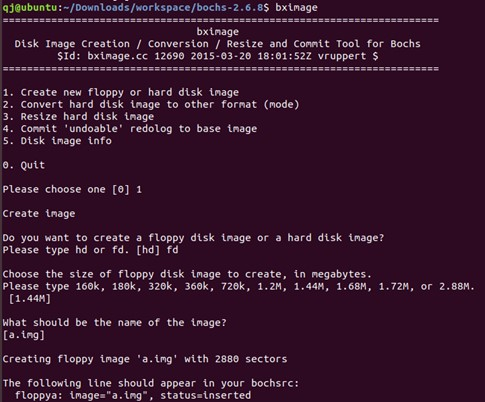
\includegraphics[width=0.7\textwidth]{figures/chapter3/3-1.jpg}
  \caption{bximage操作界面}
  \label{fig:1}
\end{figure}

创建完软盘映像后,需要编译源代码,输入以下命令即可完成编译。
\begin{lstlisting}[language = bash]
  \nasm boot.asm -o boot.bin
\end{lstlisting}

完成编译之后,我们需要使用软盘绝对扇区读写工具将这个文件写到一张空白软盘的第一个扇区,输入以下代码即可完成读入。
\begin{lstlisting}[language = bash]
  \dd if=boot.bin of=a.img bs=512 count=1 conv=notrunc
\end{lstlisting}
一切准备就绪之后,需编写 Bochs 的配置文件 bochsrc.disk,即告诉 Bochs 对虚拟机中内存,硬盘映像和软盘映像等的配置信息:\par
\# what disk images will be used\par
floppya: 1$\_$44=a.img, status=inserted\par
\# choose the boot disk.\par
boot: a\par

上述步骤完成之后,一切准备就绪,正式进行调试,输入命令:
\begin{lstlisting}[language = bash]
  \bochs -f bochsrc
\end{lstlisting}
按下回车键,再选择6,会出现如下图 3-2 所示的界面。
\begin{figure}[H]
  \centering
  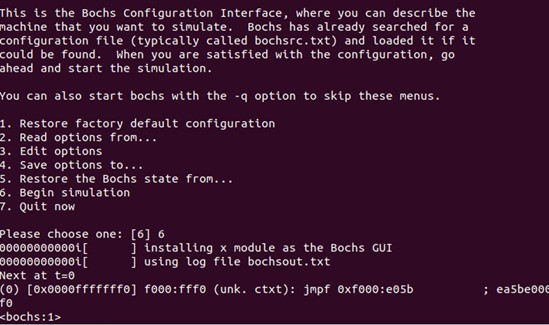
\includegraphics[width=0.7\textwidth]{figures/chapter3/3-2.jpg}
  \caption{调试过程}
  \label{fig:2}
\end{figure}

输入 c,即会进入 bochs 页面,这时,屏幕的左上角会出现一行红色的“Hello, OS world!”,即代表调试成功。调试结果如下图 3-3 所示。
\begin{figure}[H]
  \centering
  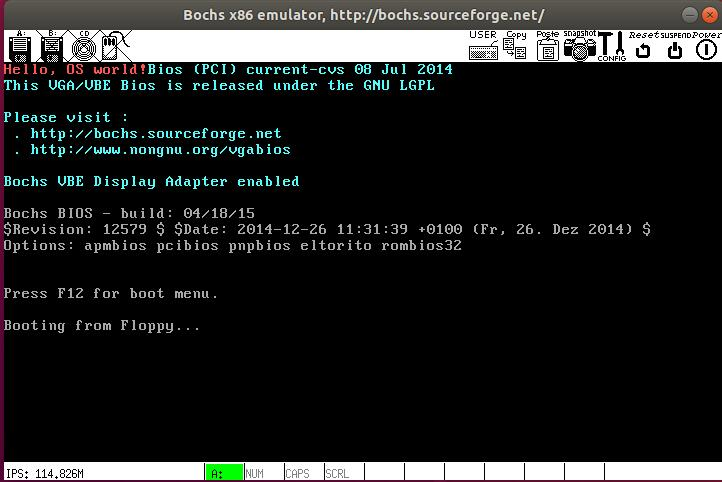
\includegraphics[width=0.8\textwidth]{figures/chapter3/3-3.jpg}
  \caption{调试结果}
  \label{fig:3}
\end{figure}

\section{实验总结}
在本实验中,我们编写了一个最简单的“操作系统”,并且使用 Bochs 软件进行仿真。但是事实上,我们编写的程序只是一个最简单的引导扇区,之所以可以称之为最简单的操作系统,是因为它可以直接在裸机上运行。计算机电源打开时,首先会加电自检,然后寻找启动盘,如果是选择从软盘启动,计算机就会检查软盘的 0 面 0 磁道 1 扇区,如果发现它以 0xAA55 结束,那么 BIOS 就会认为它是一个引导扇区。\par
当然,一个正确的引导扇区除了以 0xAA55结束之外,还应该包含一段少于 512 字节的执行码。而一旦 BIOS 发现了引导扇区,就会将这 512 字节的内容装载到内存地址 0000:7c00 处,然后跳转到 0000:7c00 处,将控制权彻底交给这段引导代码。至此为止,计算机不再由 BIOS中固有的程序来控制,而是变为由操作系统的一部分来控制。我们编写的代码中第一行就是将程序加载到 0x7c00 处,第十八行是让代码以 0xAA55 结束,因而可以作为一个独立的引导扇区运行。\par
总而言之,第二个实验的任务是一个最小的操作系统,也就是在虚拟机上运行 Helloworld。首先是 nasm 的编译,编译.asm 变为.bin,可以制作引导扇区,编译变为.com,可以调试。之后是 dd 命令写入磁盘,主要是 dd if=boot.bin of=/dev/fd0 bs=512 count=1 conv=notrunc(防止截断)。软盘读写工具将文件写到空白软盘的第一个扇区,然后让 ds 和es 两个段寄存器指向与cs 相同的段,调用子程序显示字符串,然后无限循环。最后是 bochs 的用法,用 bximage 命令创建一个空白映像文件,再使用 dd 命令将.bin 文件写入,撰写一个 bochsrc 文件,指定从软盘启动,并且使用.bin 文件。启动后使用以下命令进行调试:b 设置断点, c 继续执行, dump$\_$cpu查看寄存器, x 查看内存, n 运行下一条指令。实验二思维导图如下图3-4所示:
\begin{figure}[H]
  \centering
  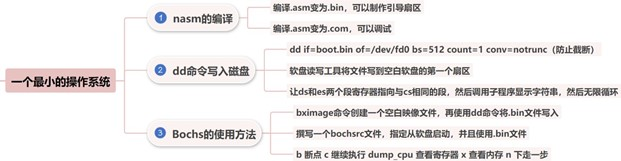
\includegraphics[width=0.8\textwidth]{figures/chapter3/3-4.jpg}
  \caption{实验二思维导图}
  \label{fig:3}
\end{figure}

 \vfill